\documentclass[tikz]{standalone}

\usepackage{tikz}
\usepackage{standalone}

\begin{document}
    \begin{tikzpicture}
        \node (nantes) at (0,0) {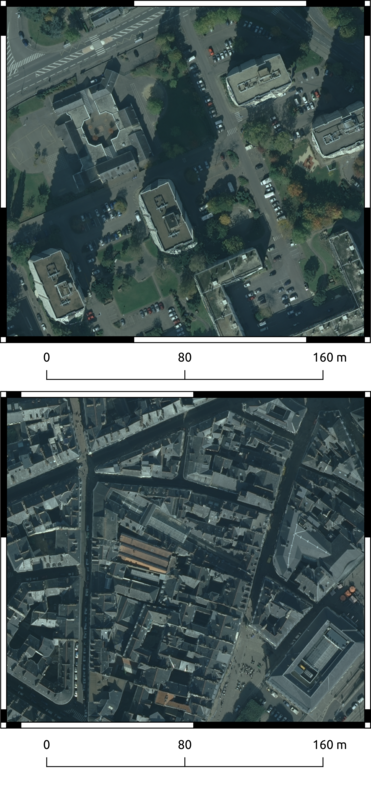
\includegraphics[height=12cm]{images/nantes}};
        \path (nantes.south) + (0, -0.5) node (nantes_l) {\large (b) Nantes};
        \path (nantes.west) + (-4, 0) node (elancourt) {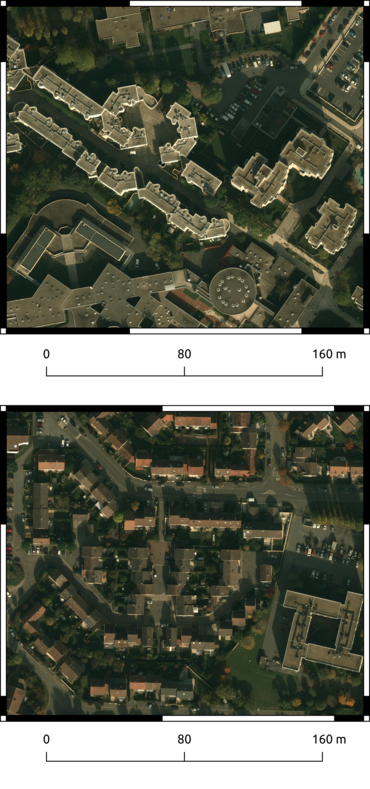
\includegraphics[height=12cm]{images/elancourt}};
        \path (elancourt.south) + (0, -0.5) node (elancourt_l) {\large (a) Elancourt};
        \path (nantes.east) + (4, 0) node (paris13) {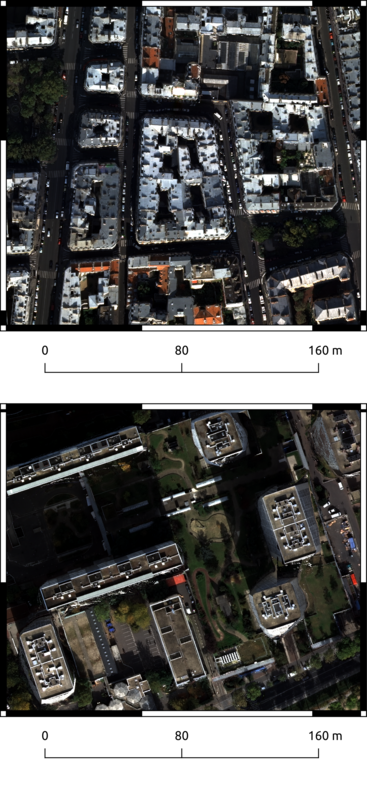
\includegraphics[height=12cm]{images/paris-13}};
        \path (paris13.south) + (0, -0.5) node (paris13_l) {\large (c) Paris-13};
    \end{tikzpicture}
\end{document}